\documentclass[brazil,times]{abnt}
\usepackage[T1]{fontenc}
\usepackage[utf8]{inputenc}
\usepackage{url}
\usepackage{graphicx}
%\usepackage{hyperref} 

\makeatletter
\usepackage{babel}
\makeatother
\begin{document}

\autor{Pedro Paulo Vezzá Campos}

\titulo{Relatório de visita ao NPD}

\comentario{Trabalho apresentado para avaliação na disciplina INE5414, do
curso de Bacharelado em Ciências da Computação, turma 04208, da Universidade   
Federal de Santa Catarina, ministrada pelo professor Carlos Becker Westphall}

\instituicao{Departamento de Informática e Estatística \par Centro
Tecnológico \par Universidade Federal de Santa Catarina}

\local{Santa Catarina - SC, Brasil}

\data{21 de agosto de 2010}

\capa

\folhaderosto

% \tableofcontents

%\chapter{}
\section*{Introdução}
I Núcleo de Processamento de Dados (NPD) pode ser considerado o ``centro
nervoso'' da UFSC. Suas atribuições incluem a administração dos recursos centrais de Processamento de
Dados da UFSC, prestação de treinamento e consultoria na área de Informática,
gerenciamento da rede local da UFSC, desenvolver e manter os sistemas
administrativos e de apoio acadêmico, dentre outros.\cite{home-setic}

\section*{Rede Nacional de Ensino e Pesquisa}
A Rede Nacional de Ensino e Pesquisa é uma rede de pesquisa com a missão de
desenvolver redes avançadas, sob a coordenação do programa interministerial do
Ministério da Educação e Ministério das Ciências e Tecnologia. Equivalentes em
outros países incluem a Internet2 (EUA) ou a Renater (França).\cite{apresentacao-rnp}

\begin{figure}[htp]
\begin{center}
  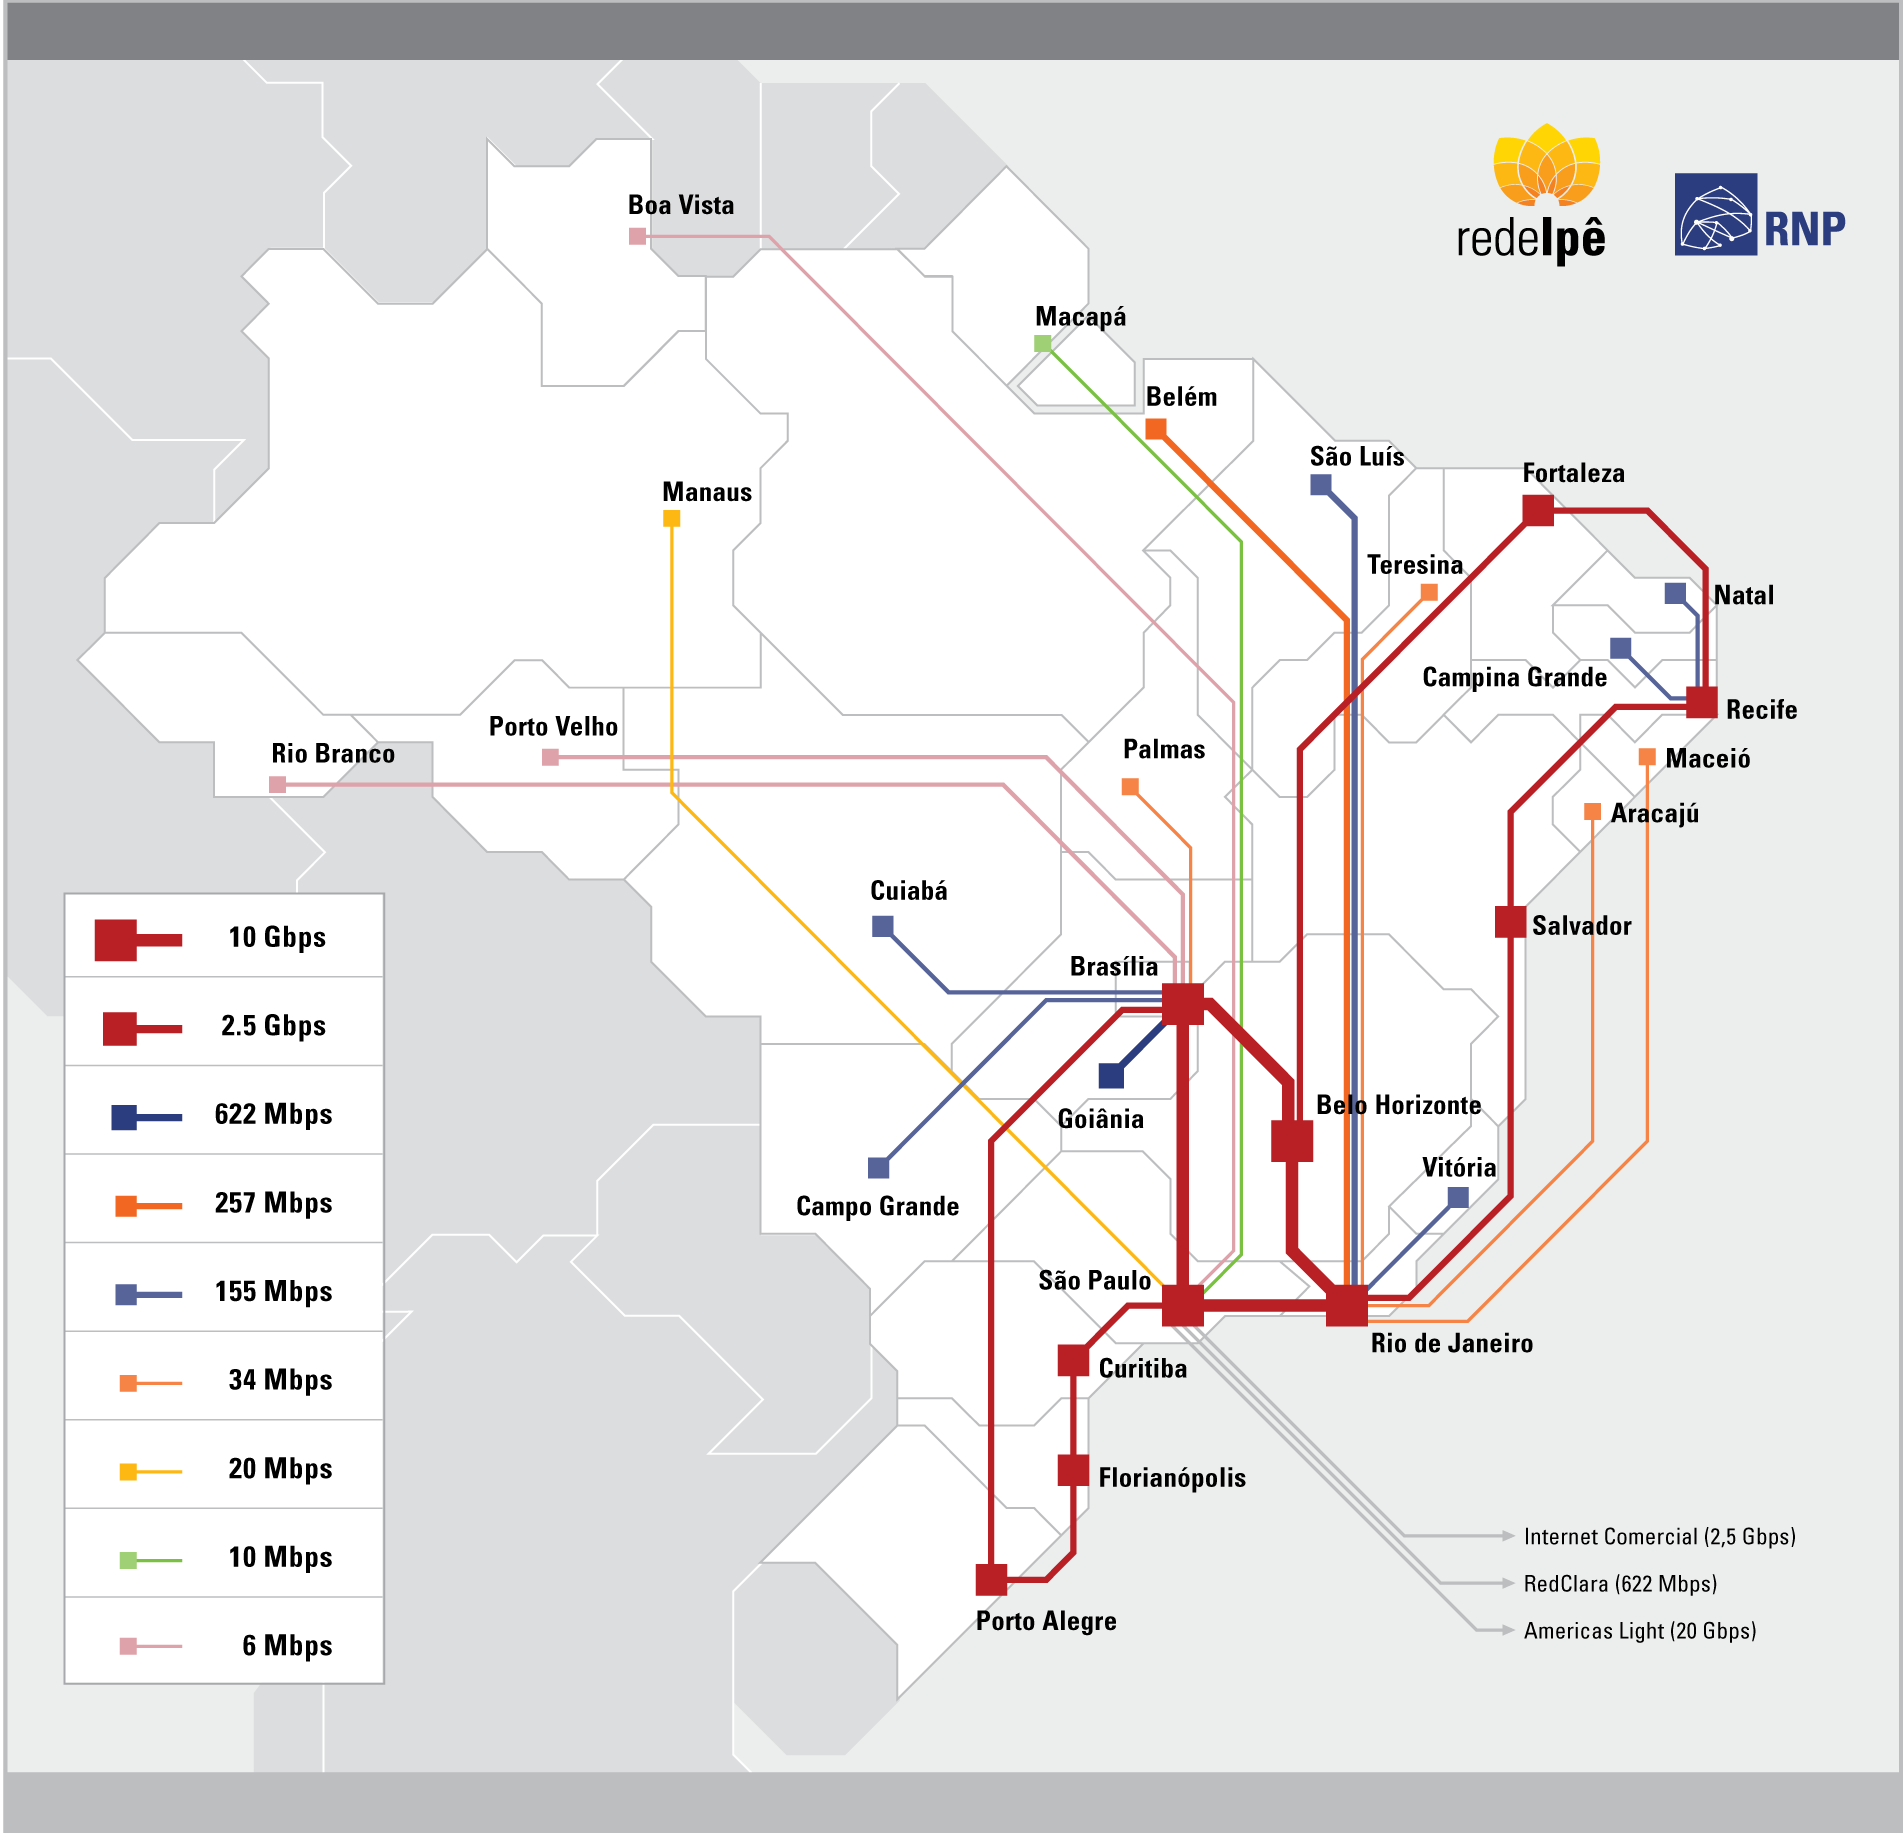
\includegraphics[width=110mm]{imagens/backbone-rnp-201005.png}
  \caption[Mapa do backbone atual da RNP]{Mapa do backbone atual da RNP}
  \label{backbone-rnp}
\end{center}
\end{figure}

No Brasil, a rede Ipê (Figura \ref{backbone-rnp}) é a infraestrutura da RNP de
Internet voltada para a comunidade brasileira de ensino e pesquisa. Através dela conectam-se as
principais universidades e institutos de pesquisa do país.\cite{home-rnp}

Alguns serviços fornecidos pela RNP incluem:
\begin{itemize}
  \item Internet de alta velocidade e disponibilidade
  \item Fone@RNP: Serviço de VoIP
  \item Vídeo conferência em alta definição
  \item Repositório de vídeos e transmissão de sinal de TV, dentre outros.
\end{itemize}

\section*{Rede Metropolitana da Região de Florianópolis}
A Rede Metropolitana da Região de Florianópolis (REMEP-FLN) abrange
Florianópolis, São José e Palhoça. Sua responsabilidade é de interconectar
diversas universidades e entidades, dentre elas a UFSC, Udesc, Unisul, CIASC,
CIDASC, EPAGRI. \cite{apresentacao-remep}

%\usepackage{graphics} is needed for \includegraphics
\begin{figure}[htp]
\begin{center}
  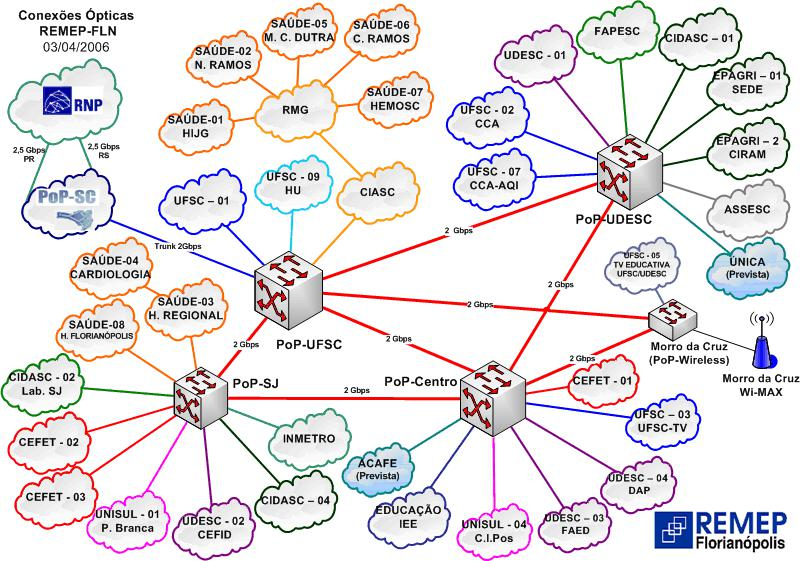
\includegraphics[width=110mm]{imagens/remep.jpeg}
  \caption[Panorama da REMEP-FLN]{Panorama da REMEP-FLN}
  \label{mapa-remep}
\end{center}
\end{figure}

Na UFSC encontra-se a ligação entre a REMEP e o Pop-SC, como pode ser visto na
imagem abaixo. É através dela que a rede possui conectividade com a Intenet,
habilitando-se a fornecer serviços de VoIP, vídeo conferência, transmissão de
imagens médicas (telemedicina), transmissão ao vivo de TVs como a TV UFSC,
Unisul e Cultura, transmissão de grandes volumes de dados para metereologia,
etc. \cite{apresentacao-rnp}


\section*{POP-SC}
O Ponto de Presença (POP) em Santa Catarina da Rede Nacional de Pesquisa (RNP)
localiza-se na UFSC. Instituições governamentais e de pesquisa catarinenses
conectam-se à Internet através do POP-SC. Atualmente a infra estrutura
constitui-se de duas ligações, uma para o Rio Grande do Sul e outra para o
Paraná, cada uma delas com uma taxa de velocidade de 2,5Gbps. Há planos de
expansão para 10Gbps.

\begin{figure}[htp]
\begin{center}
  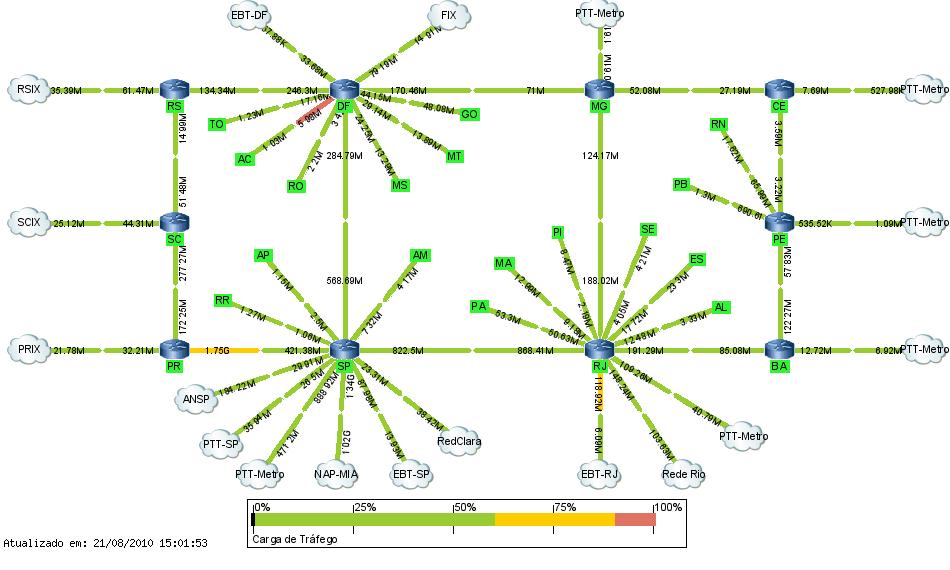
\includegraphics[scale=0.48]{imagens/panoramaRNP.png}
  \caption[Panorama da RNP mostrando as duas ligações de Santa
  Catarina com o Paraná e Rio Grande do Sul]{Panorama da RNP mostrando as duas ligações de Santa
  Catarina com o Paraná e Rio Grande do Sul}
  \label{panorama-rnp}
\end{center}
\end{figure}

\section*{Ponto de Troca de Tráfego}
Pontos de Troca de Tráfego são locais onde diversas redes diferentes podem
trocar tráfego de maneira gratuita. Essa abordagem traz a vantagem de reduzir
custos e aumentar o desempenho das redes pois balanços de tráfego são resolvidos
direta e localmente e não através de redes de terceiros, muitas vezes
fisicamente distantes. \cite{ptt-metro}

Na UFSC encontra-se o PTT de Santa Catarina, interligando redes de provedores
comerciais como Linha Livre, NET, Newsite, dentre outros a órgãos governamentais
como CIASC, RNP e NIC-BR.\cite{ptt-participantes}
 
\section*{redeUFSC}
O NPD é responsável pela manutenção da rede interna da UFSC.
Para isso, há uma infraestrutura especial para manter os switches que interligam
os diferentes centros e departamentos da universidade. Em uma sala encontram-se
os switches do POP-SC e REMEP-FLN, que pode ser vista na figura
\ref{sala-racks}. É por essa sala que deve passar todo o tráfego de entrada ou
saída da Rede Nacional de Pesquisa, ao centro da da figura \ref{sala-racks} é possível
ver o switch Juniper que faz a interligação de Santa Catarina com a RNP através
de duas ligações de fibra ótica, uma com o Paraná e outra com o Rio Grande do
Sul, cada uma com 2,5 Gbps.

Já em outra sala encontram-se diversos servidores, como os de
VoIP, VPN, WWW, etc. Diversos desses servidores foram virtualizados
utilizando-se tecnologia VMware, o que permite uma economia de custos, já que os
mesmos serviços podem ser oferecidos utilizando-se um número menor de máquinas,
economizando-se em energia elétrica, equipamentos e espaço.

Na figura \ref{backbone-ufsc} é representado o backbone principal da UFSC em
2010. Nela são apresentados os dois roteadores Cisco da universidade (NPD[252]
e NPD[253]). Conectados a eles encontram-se diversos switches de diversas
marcas espalhados pelos diversos centros e departamentos, alguns desses switches
estão representados na figura.

Claramente o NPD desempenha papel central na administração da redeUFSC. Tal
arquitetura de rede por um lado facilita a manutenção pois diversos serviços
estão concentrados em um único local, por outro lado, ele pode ser visto como
um ``elo fraco'' na rede uma vez que um comprometimento nesse ponto pode afetar
de maneira drástica toda a rede da universidade.

%\usepackage{graphics} is needed for \includegraphics
\begin{figure}[htp]
\begin{center}
  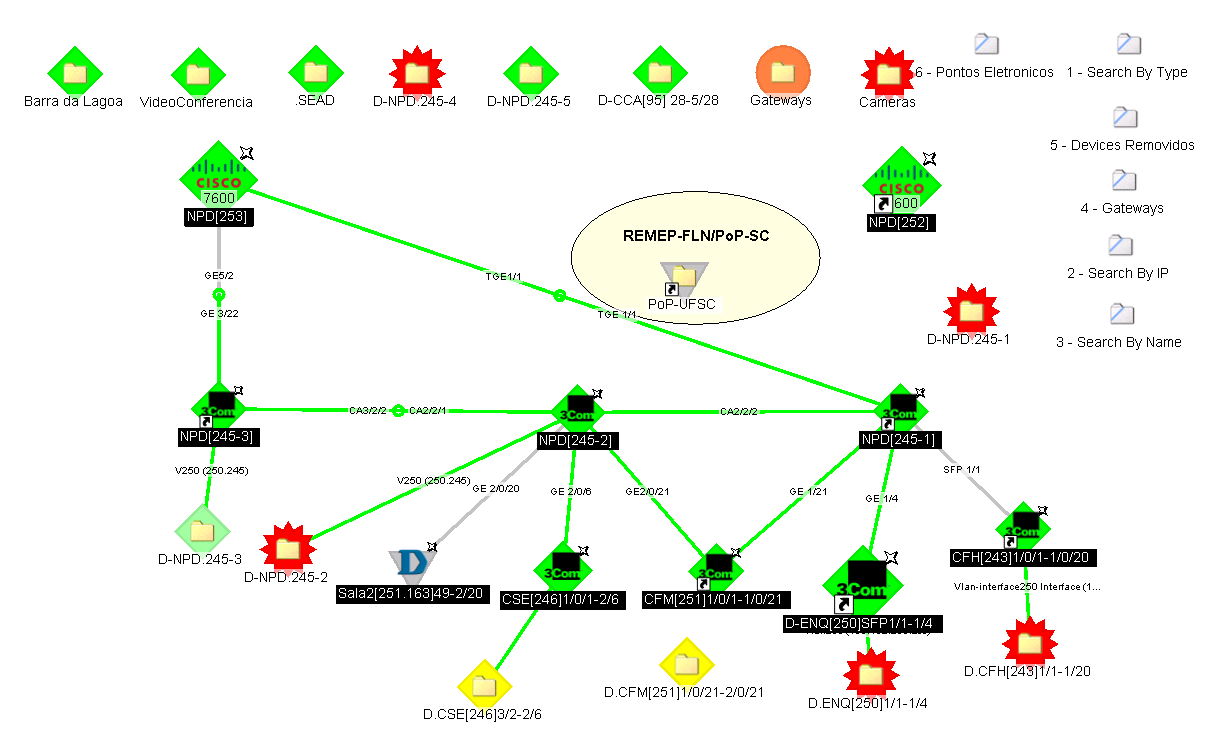
\includegraphics[width=150mm]{imagens/Topo-Mapa.png}
  \caption[Backbone da UFSC em 2010]{Backbone da UFSC em 2010}
  \label{backbone-ufsc}
\end{center}
\end{figure}

Ambas as salas contam com um ambiente refrigerado para melhor funcionamento dos
equipamentos, além de um piso levantado, que evita possíveis problemas com
alagamentos e facilita o cabeamento entre racks. Parte das instalações é
redundante para controlar possíveis interrupções no funcionamento normal dos
equipamentos.

A Universidade ainda conta com a RedeUFSCSemFio, uma rede de \emph{Access
Points} espalhados pela universidade que fornecem conectividade sem fio a
estudantes, funcionários e visitantes.

\begin{figure}[htp]
\begin{center}
  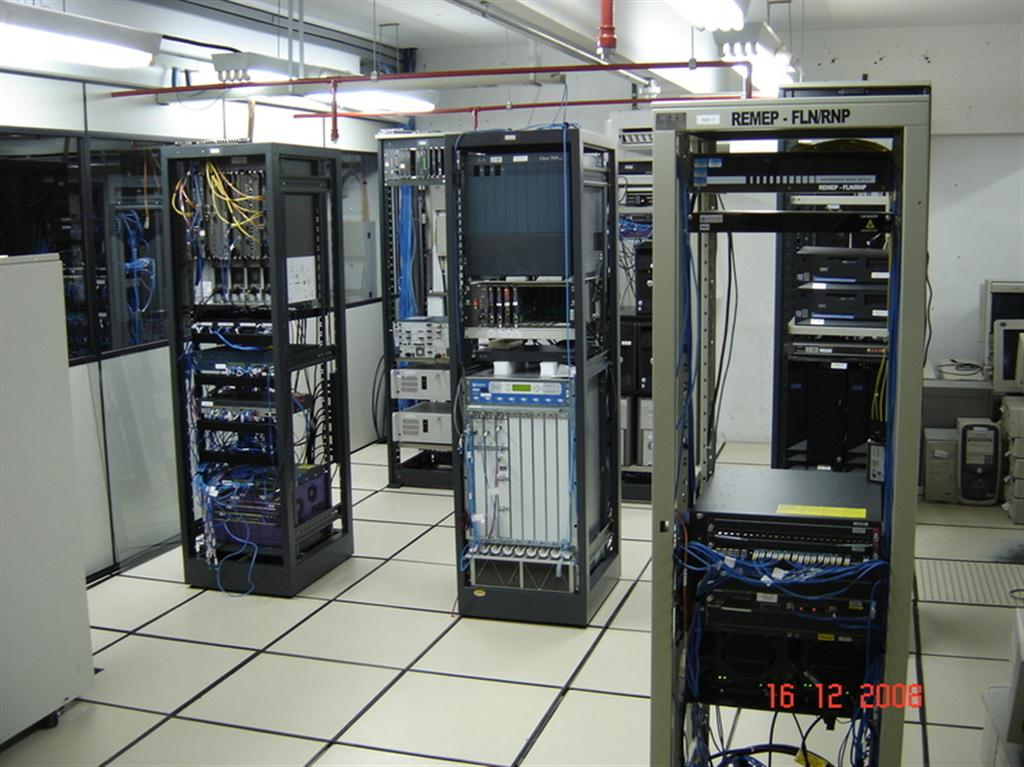
\includegraphics[width=110mm]{imagens/sala-racks-setic.jpeg}
  \caption[Sala com os Racks do POP-SC e REMEP-FLN]{Sala com os Racks do POP-SC
  e REMEP-FLN}
  \label{sala-racks}
\end{center}
\end{figure}
% 
% \section*{Rede INF}
% A Rede INF é a rede interna do Departamento de Informática e Estatística da
% UFSC. É através dela que os alunos e professores do departamento possuem acesso
% a serviços de e-mail, hospedagem de páginas web estáticas e dinâmicas, banco de
% dados MySQL, SVN etc. \cite{redeinf-pet}
% 
% Os alunos possuem atualmente acesso a dois servidores UNIX:
% \texttt{venus.inf.ufsc.br e marte.inf.ufsc.br}. É neles que hospedam-se as
% páginas web do departamento além do uso de algumas ferramentas de console, como
% o GCC. \cite{redeinf-pet}
% 
% Para acessar a Internet, o tráfego de de rede do departamento deve percorrer o
% seguinte caminho: Da máquina de origem deve rumar até a sala de Administração da
% Rede INF (AdmRede) no terceiro andar do departamento, depois deve seguir até um
% dos switches da SeTIC, por fim atingindo o switch principal do POP-SC, que se
% interconecta com a RNP e a Internet comercial.

\bibliographystyle{abnt-num}
\bibliography{referencias}
\end{document}